\chapter{Absorption of Beta and Gamma Rays}
\textbf{Objective:} To study the behavior of gamma and beta rays passing through matter; to measure the range of beta-particles from a given source and hence to determine the endpoint energy of decay; to determine the absorption coefficient in lead of the gamma radiation from a given source.\myskip

\textbf{Safety Note:} The radioactive sources used in this experiment are extremely weak and therefore can be handled without any danger of overexposure to radiation. However, it is always prudent not to handle any radioactive source more than is necessary.

\section{Discussion}
All nuclei heavier than lead (and many isotopes of lighter nuclei) have a finite probability of decaying spontaneously into another nucleus plus one or more lighter particles. One of the decay products may be an alpha-particle (two protons and two neutrons--the stable nucleus of a helium atom). Alternatively, a nucleus with more neutrons than it can maintain in stability may decay by emission of an electron from the nucleus (beta-decay) which corresponds to the conversion of a neutron to a proton. These electrons may emerge with a kinetic energy of up to several MeV.\myskip
\begin{figure}[h]
\centering
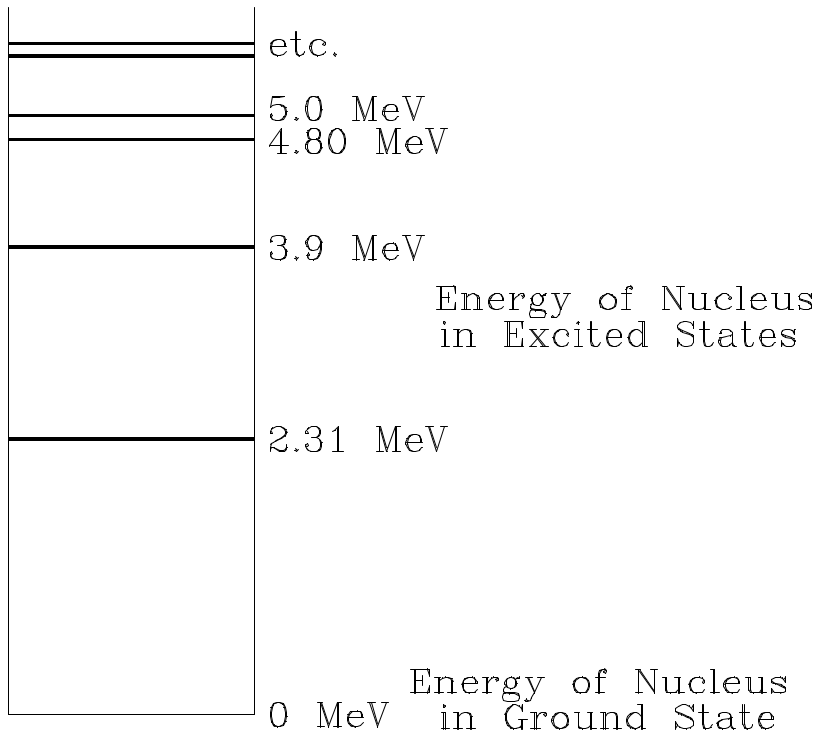
\includegraphics[width=0.5\textwidth]{./Exp10/pic/image1.png}
\caption{Typical Nuclear Energy Level Diagram.}
\label{fig:level}
\end{figure} 

After alpha or beta decay, the residual nucleus may be left in an excited state. In this case, a transition to a state of lower energy of the same nucleus will occur almost immediately with the emission of a photon (gamma ray). The spectrum of photons emitted from the various excited states of a nucleus will have discrete frequencies $\nu$, corresponding to transitions $\Delta E=h\nu$, between discrete energy levels of the nucleus. The gamma ray spectrum from an excited nucleus is thus \textbf{analogous} to the line spectrum of visible radiation from an atom due to excited electrons, with the notable difference that the MeV energy changes of the nucleus are approximately $10^6$ times as large as energy changes in transitions between atomic states (where $\Delta E_{\mathrm{atomic}}\approx$ several eV). See Figure {\ref{fig:level}}.\myskip
\begin{figure}[h]
\centering
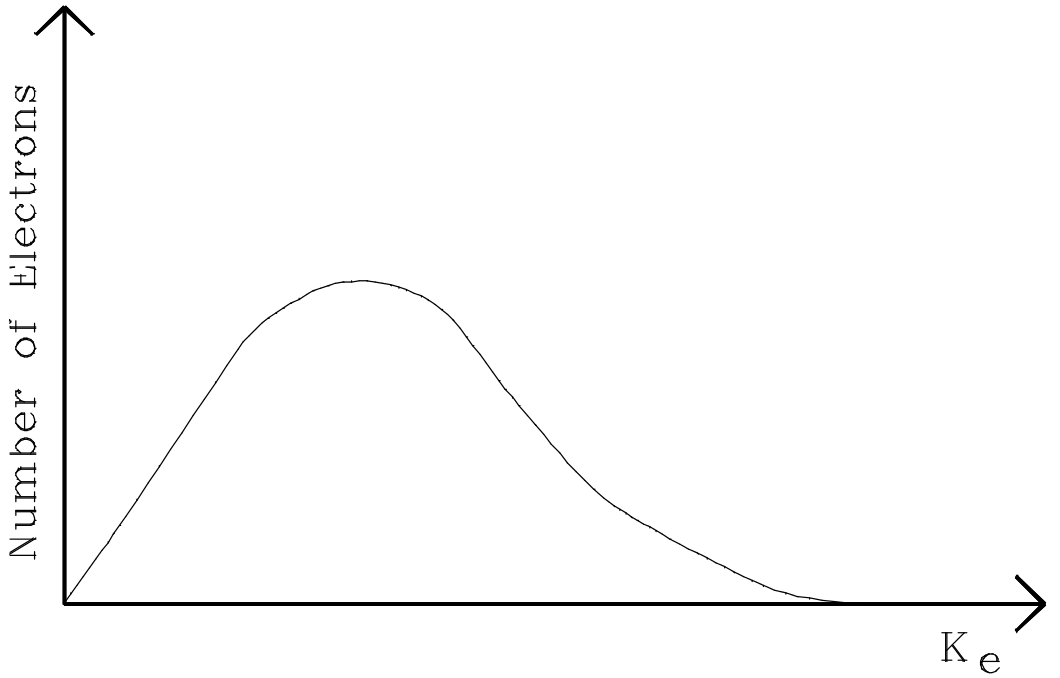
\includegraphics[width=0.5\textwidth]{./Exp10/pic/image2.png}
\caption{Beta Ray (Electron) Energy Spectrum}
\label{fig:betaray}
\end{figure} 

In early experiments on beta-decay, it was observed that each decay was not a simple one in which an electron and the recoil nucleus came off with equal and opposite momentum. The electrons, in fact, were emitted with a continuous spectrum of energies (Figure {\ref{fig:betaray}}). It was subsequently suggested by Pauli and Fermi that in each decay, another particle of zero mass and charge, called the neutrino, was emitted. Experimental verification of the neutrino has been obtained by observation of its rare interaction with matter.


\section{Detection of Charged Particles (the Geiger Counter)}
When an energetic charged particle traverses matter, it will give electrostatic impulses to nearby electrons and thus ionize atoms of the material. Most methods for detecting nuclear particles rely on observing the results of this ionization. In a photographic emulsion, a trail of ionized grains will show up when the film is developed. A trail of droplets or bubbles forms along the wake of ionization left by a charged particle passing through a cloud or bubble chamber. In a scintillation counter, ionized molecules will very rapidly radiate visible light. A charged electroscope will be discharged by ion pairs created in air. In the \textbf{geiger counter}, which will be used as a detector in this experiment, the ionization produced by a charged particle causes a violent electrical discharge.
\begin{figure}[h]
\centering
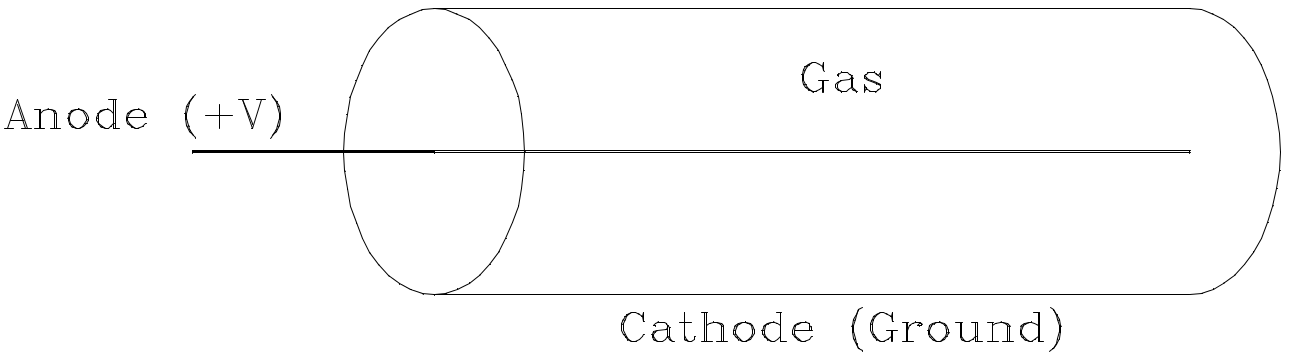
\includegraphics[width=0.5\textwidth]{./Exp10/pic/image3.png}
\caption{The Geiger Counter.}
\label{fig:counter}
\end{figure} 

As shown in Figure {\ref{fig:counter}}, the counter consists of a metal cylinder (cathode) with insulating ends supporting a fine axial wire (anode). When a charged particle ionizes the gas (e.g., argon) in the tube, electrons will move toward the positively charged anode wire, accelerated more and more by the rapid increase in electric field near the wire. When an electron acquires kinetic energy greater than the ionization energy of the gas molecules, it can create by collision a new ion and electron, which in turn can accelerate and create another ion, etc., thus initiating an avalanche of charge. The process, called the \textbf{Townsend avalanche}, is possible only if the voltage maintained between anode and cathode is sufficiently high.\myskip

The basic counter circuit, shown in Figure {\ref{fig:geiger}}, supplies a positive high voltage of up to 900 volts to the center wire. When an avalanche occurs, current flows through $R$, the counter side of $R$ drops in potential, and this negative pulse is fed through $C$ to a stage of amplification and then to a scaling device.
\begin{figure}[h]
\centering
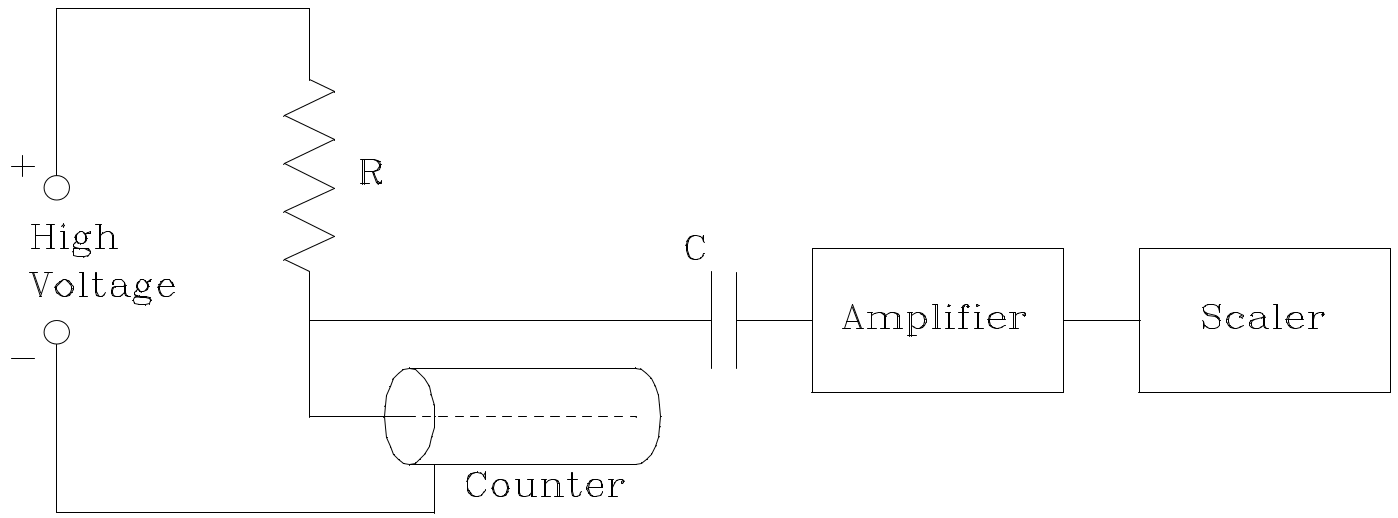
\includegraphics[width=0.8\textwidth]{./Exp10/pic/image4.png}
\caption{Geiger Counter Circuit.}
\label{fig:geiger}
\end{figure} 

For a large enough value of $R$, the voltage drop across R would be sufficient to stop the discharge after a count has been recorded. This method of quenching the discharge,
however, has the disadvantage of creating a long time constant, $\tau = RC$, for reestablishing voltage across the counter, i.e., of creating a long ``dead time'' during which the passage of another particle cannot be detected. The quenching can be achieved for a lower value of $R$ by adding halogen vapor to the gas to help absorb ion pairs. Nevertheless, the resultant dead time is substantial and must be taken into account when the particle flux is high.

\section{Energy Loss and Range of Beta Particles}
Because of its ionizing action (Figure {\ref{fig:ionizing}}), a \emph{charged}, incident particle in matter will continuously lose kinetic energy, and the particle will subsequently come to rest after traversing a path length called its \textbf{range}. \emph{For a particle of known charge and mass, there will be a unique range associated with each incident energy}. A formula can be theoretically deduced for the rate of energy loss--and hence the range--of a particle (of known mass, charge, and initial velocity) in a particular ``stopping'' material (of known electron density and ionization potential).
\begin{figure}[h]
\centering
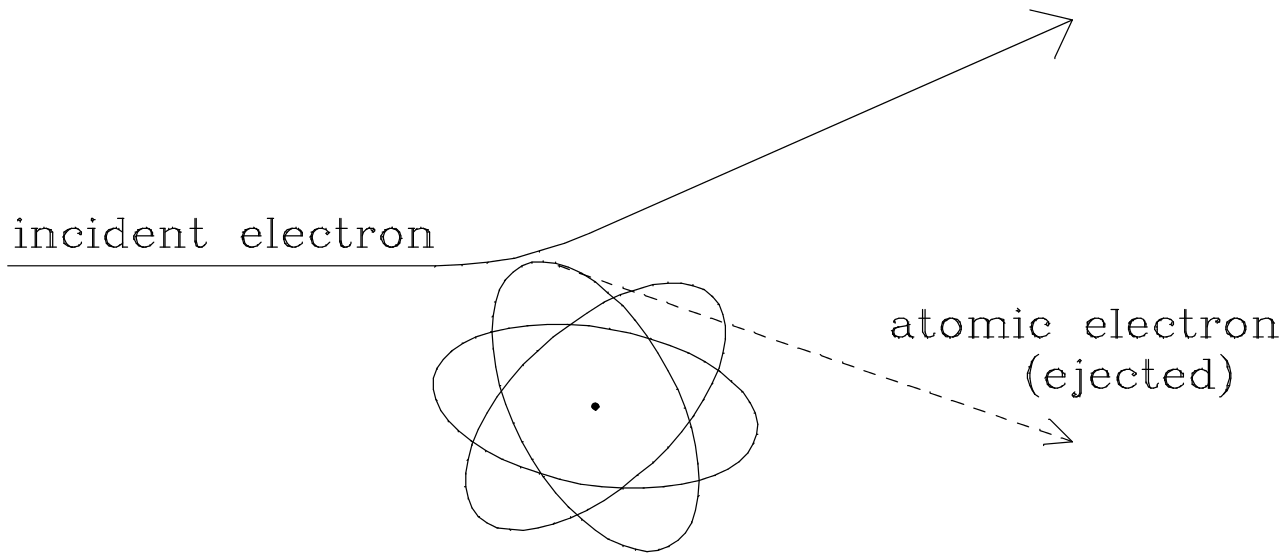
\includegraphics[width=0.5\textwidth]{./Exp10/pic/image5.png}
\caption{Ionizing Action of Incident Electron.}
\label{fig:ionizing}
\end{figure} 

In each interaction with atomic electrons, however, an incident electron may be scattered through small or relatively large angles, and as it traverses the material it may follow a rather tortuous, winding path (especially at low energies). Therefore, the actual path of the electron may be considerably longer than the observed distance that it penetrates into the material. For this reason, the incident electron range is not sharply determined, and the theoretical calculation is of limited usefulness for electrons of less than $1\, \mathrm{MeV}$ energy.\myskip

In this experiment, therefore, we will use an approximate empirical relationship between range and energy for low energy electrons:
\begin{equation}
  r=\frac{0.412\, \mathrm{g}/\mathrm{cm}^2}{\rho}E^{1.29}
\label{eq:re}
\end{equation}
where $r$ is in cm, $E$ is in MeV, and $\rho$ is the density of the stopping material in $\mathrm{g} / \mathrm{cm}^3$. Note that the density of Aluminum is $2.702\,\mathrm{g} /\mathrm{cm}^{3}$.\myskip

(This result is described in: L. Katz and A. S. Penfold, ``Range-Energy Relations for Electrons and the Determination of Beta-Ray End-Point Energies by Absorption,'' Revs.Modern Phys. \textbf{24}, 1 (1952).)

\section{Absorption of Gamma Rays}
Gamma rays, or high-energy photons, can interact with matter by three distinct processes:
\begin{enumerate}[1)]
\item Compton Scattering: This refers to a photon-electron collision in which the energy lost by the scattered photon is given to the recoil electron.
\item Photoelectric Effect: The photon is absorbed by the atom as a whole, releasing an electron with kinetic energy equal to $E_{\gamma} - E_{b}$ , where $E_{\gamma}$ is the photon energy and $E_{b}$ is the relatively small binding energy of the electron in the shell from which it is released.
\item Pair Production: If the photon has energy greater than $1.02\, \mathrm{MeV}$, it can create an electron-positron pair in the neighborhood of a nucleus. The radiative source used in this experiment does \textbf{not} emit photons with energy greater than $1\, \mathrm{MeV}$. 
\end{enumerate}

The probability of each of the three processes taking place in a given thickness of material depends on the energy of the photon and the atomic structure of the material. The \emph{total} probability for interaction of photons in Pb, i.e., the sum of the probabilities of the three processes, varies with photon energy as indicated in Figure {\ref{fig:linear}}. The ordinate plotted on the graph is $\mu$, the \textbf{total linear absorption coefficient} in units of $\mathrm{cm}^{-1}$. It is defined by the equation:
\begin{equation}
  \frac{d N}{d x}=\mu N
\end{equation}
where $N$ is the number of incident photons and $dN$ is the number removed from the beam (i.e. absorbed) in an absorber of thickness $dx$ (in cm). Note that $dN$ and $dx$ are the calculus equivalents of infinitesimally small values of $\Delta N$ and $\Delta x$, respectively. As in any process where the rate of decrease is proportional to the number present (such as the discharge of a capacitor), the solution of this differential equation is:
\begin{equation}
  N(x)=N_{0}e^{-\mu x}
\label{eq:nx}
\end{equation}
where $N(x)$ is the number of photons passing through $x\,\mathrm{cm}$ of absorber and $N_0=N(x)$ at $x = 0$ , and $e$ is the base of natural logarithms.
\begin{figure}[h]
\centering
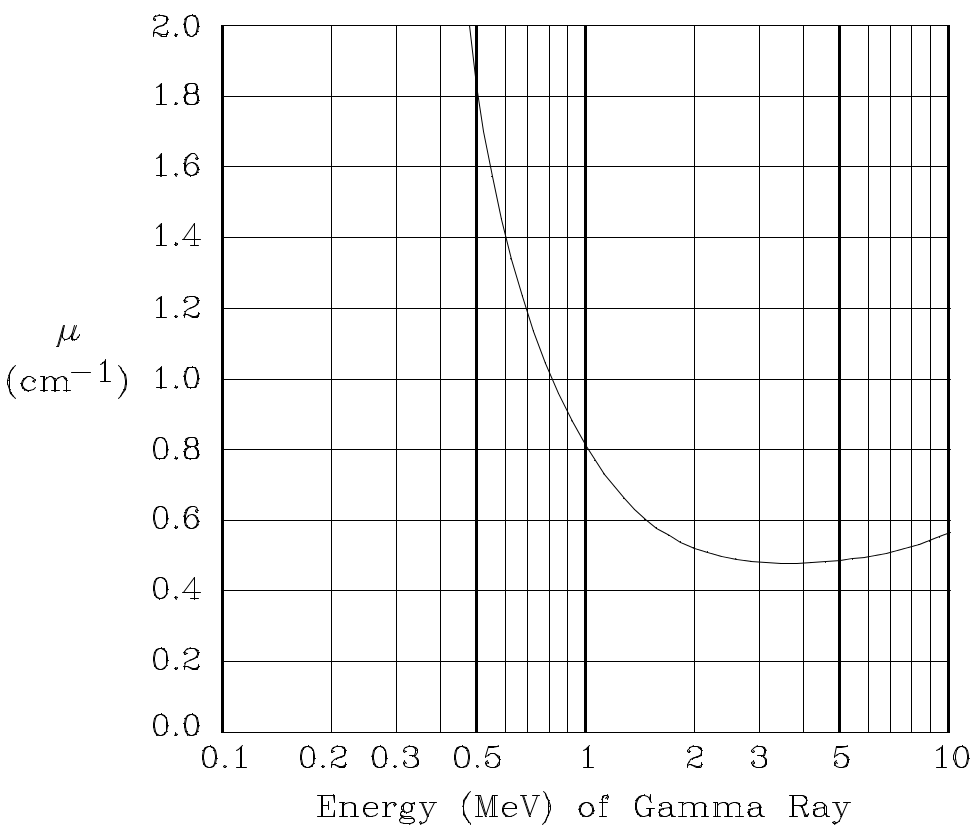
\includegraphics[width=0.8\textwidth]{./Exp10/pic/image6.png}
\caption{Linear Absorption Coefficient μ for gamma rays in lead as a function of energy.}
\label{fig:linear}
\end{figure} 

\section{Procedure}
\subsection{Adjustments and Measurement of Errors in Counting}
\subsubsection{High Voltage Variations}

Every Geiger tube that is in good working order has a plateau region in which its counting rate is relatively insensitive to changes in the high voltage supply. This region can be found by putting a source under the tube and increasing the high voltage from its lowest value until the tube just begins to count. One can then take 15 second counts while raising the voltage in 50 volt steps. The curve of counting rate vs. voltage levels off, i.e., the count rate rises by less than 10\% for a 100-volt increase. Do not raise the voltage furthere as this may damage the tube due to continuous breakdown. Set the high voltage to a value on this plateau for the remainder of the experiment. If this procedure is followed correctly, high voltage variations may be ignored as a source of error.

\subsubsection{Statistical Accuracy}

Particles decay randomly in time from a radioactive source (over a period short compared to the half-life). The probability distribution for measuring a given number of these counts in a given time interval is an almost bell shaped curve (a Poisson Distribution) centered around $N_0$, the most probable value. The distribution will have a standard deviation about the peak of $\pm \sqrt{N_{0}}$ . If $N$ counts are measured in an interval, the best estimate of the error is $\pm \sqrt{N}$ .\myskip

Note that the magnitude of the statistical error--your uncertainty in the measurement--increases significantly for trials involving a very small number of counts. For a high counting rate in a given interval, say, 900 counts in one minute, the estimated error will be 30 counts per minute or 3.3\% error. However, for a much lower counting rate in the same interval, say 25 counts, the error of $\pm$5 counts per minute amounts to a 20\% statistical error. In order to achieve the same precision as in the first case, it would be necessary to collect 900 counts--in other words, to take a 36-minute measurement. While such a long measurement is impractical for this lab, you should keep in mind the relationship between a small number of counts and higher errors, and do your best to minimize these errors by taking longer measurements when necessary.

\subsubsection{Measuring Background Radiation}

In order to make accurate counting measurements of the sources, it is necessary to know the counting rate due to natural background radiation (mostly cosmic rays coming through the earth's atmosphere). Additionally, there will be some excess counts due to the Cs-137 gamma sources nearby in the room, whose gamma rays can pass through the side of the detector. At a distance of $30\,\mathrm{cm}$, for example, the Cs-137 source contributes roughly as many counts as the natural background radiation (doubling the distance would reduce its contribution to one-fourth this level). It's best to try to minimize these secondary effects-- by keeping your detector far from others' sources, and by shielding your own Cesium source with the lead sheets when not in use), but it's even more important to try to keep these background effects \emph{constant}. If all of your data is shifted by roughly the same constant amount, then it is possible to isolate the results you're interested in by subtracting out this constant background.

\subsection{Range of Beta Particles}
\begin{figure}[h]
\centering
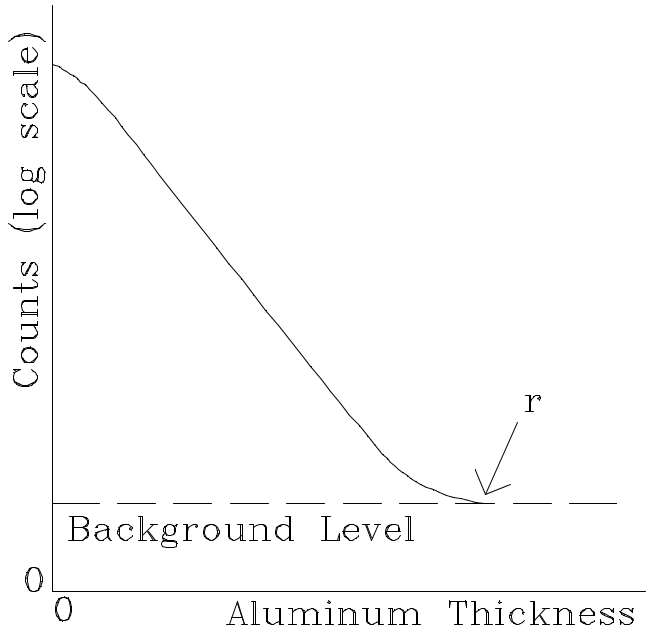
\includegraphics[width=0.4\textwidth]{./Exp10/pic/image7.png}
\caption{Beta Absorption Curve}
\label{fig:beta}
\end{figure} 
Thallium 204 beta decays to Lead 204 with a half-life of 3.9 years. The range of the most energetic of the decay electrons can be determined by placing aluminum foil absorbers between the source and the geiger counter.\myskip

A typical absorption curve is shown in Figure {\ref{fig:beta}}. The maximum range $r$ is the point where the absorption curve meets the background. You should start by making a careful measurement of background, and you should repeat this measurement after taking the absorption curve to check for constancy.\myskip

Place the Thallium source on the second shelf below the detector, as shown in Figure {\ref{fig:absorption}}, to maximize the number of counts while leaving enough room to stack aluminum absorbers. Begin taking measurements for the absorption curve, adding aluminum foils until the counting rate reaches the background level. (\emph{Note that the thickness of the aluminum absorbers is marked on the foil in \textbf{mils}, or thousandths of an inch, not millimeters}.)\myskip
\begin{figure}[h]
\centering
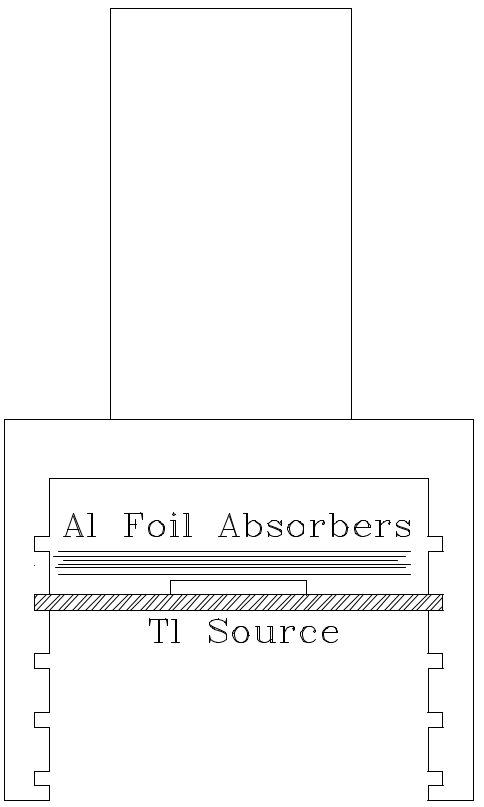
\includegraphics[width=0.25\textwidth]{./Exp10/pic/image8.png}
\caption{Beta Absorption}
\label{fig:absorption}
\end{figure} 

Make a table of the results, including the background level, and include estimates of the statistical error in each measurement. Note that you \emph{should not} subtract background from your data for this experiment. Plot the results on the semi-log paper provided (if your measurements are of different durations, you will need to scale them to a constant duration which is convenient for graphing).\myskip

Determine the approximate value of the maximum range from the graph, and use Eq. ({\ref{eq:re}}) to compare your result with the value of $0.765\ \mathrm{MeV}$ for the maximum beta energy for Thallium 204 as measured in a magnetic spectrometer. 

\subsection{Absorption of Gamma Rays}
The source for this part of the experiment is Cesium 137, which decays with a half-life of 30 years to Barium 137 with the emission of a $0.52\, \mathrm{MeV}$ beta ray (Figure {\ref{fig:cesium}}). The resulting Barium is in an excited state and decays by emitting a $0.662\, \mathrm{MeV}$ gamma ray almost instantaneously. Lead absorbers are used for the gamma absorption study. They are thick enough(0.062 inches) so that one absorber will stop all the betas.\myskip
\begin{figure}[h]
\centering
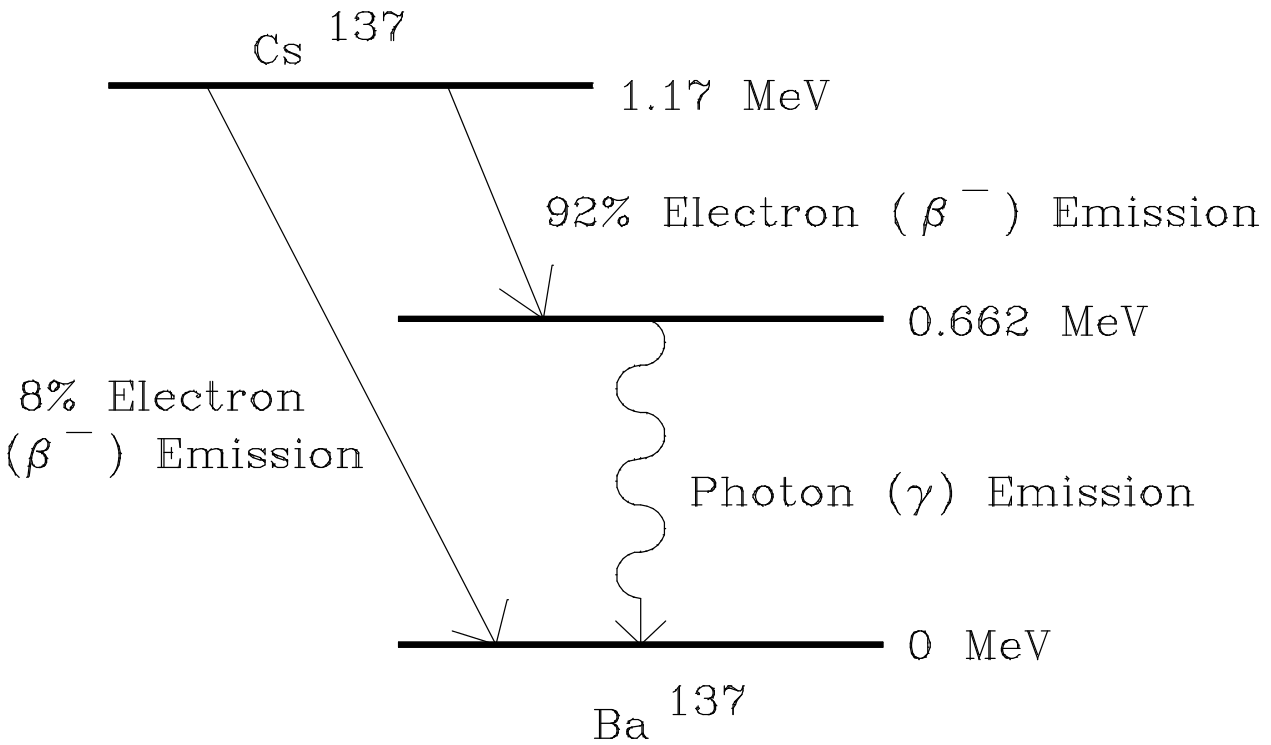
\includegraphics[width=0.5\textwidth]{./Exp10/pic/image9.png}
\caption{Cesium 137 Decay Scheme}
\label{fig:cesium}
\end{figure} 

The gamma rays are detected by means of the same geiger counter used in the previous part. Note that the efficiency of the geiger counter for detecting photons is much less than for detecting the beta rays, since it depends on a collision of the photon with the gas or wall of the counter, resulting in the emission of an electron, which in turn initiates the discharge.\myskip
\begin{figure}[h]
\centering
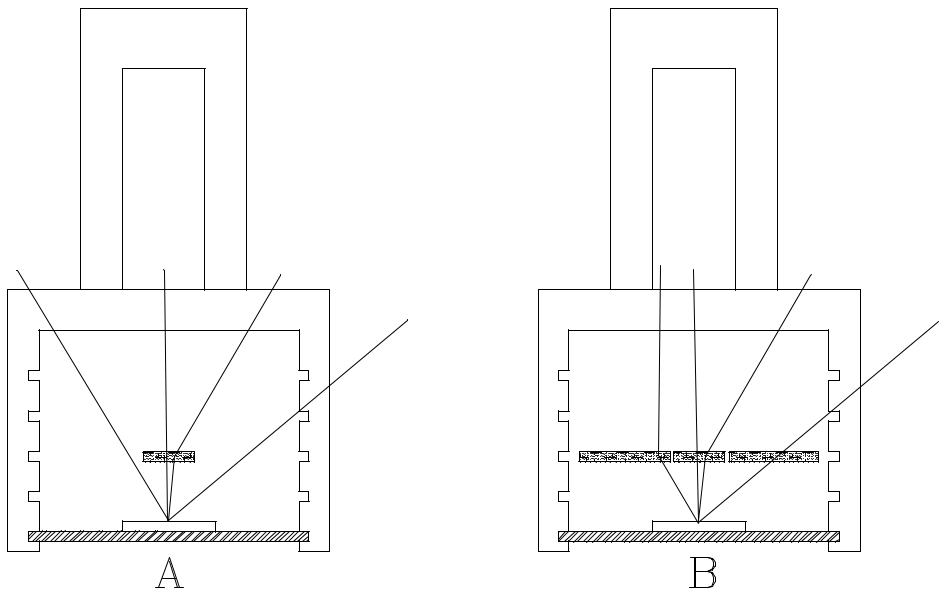
\includegraphics[width=0.5\textwidth]{./Exp10/pic/image10.png}
\caption{Scattering Effects: In (A), the gamma ray on the left passes outside of the detector tube. In (B), it can be seen how increasing the area of lead absorber can cause the same gamma ray to scatter \emph{into} the detector.}
\label{fig:scattering}
\end{figure} 

Figure {\ref{fig:scattering}} represents one of the effects of gamma ray scattering in the lead sheets. Increasing the \emph{area} of lead through which the gamma rays pass tends to \emph{increase}, rather than decrease, the number of counts one measures, since gamma rays which otherwise would not have entered the detector may now be scattered into it.\myskip
\begin{figure}[h]
\centering
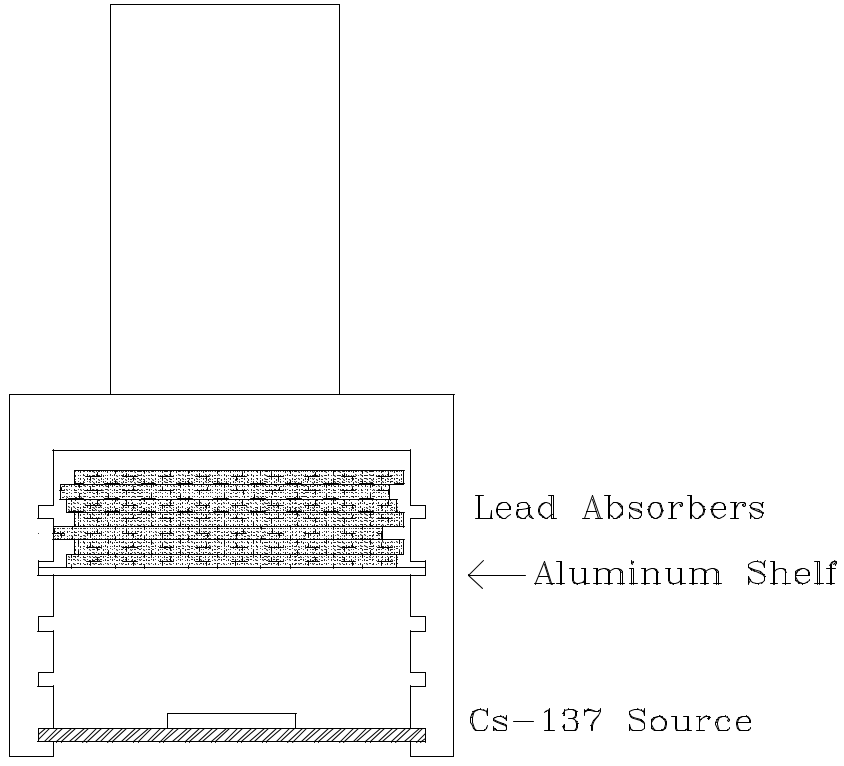
\includegraphics[width=0.4\textwidth]{./Exp10/pic/image11.png}
\caption{Absorption of Gamma Rays Set-Up.}
\label{fig:gammarays}
\end{figure} 

The arrangement shown in Figure {\ref{fig:gammarays}} is designed to reduce the effect of such scattering. By keeping the lead sheets high above the source, one reduces the excess area exposed to gamma rays, and one reduces the effective difference in area between the top and bottom sheets as well.\myskip

Take measurements for an absorption curve. Note how this differs fundamentally from beta absorption: there is no maximum range for gamma rays passing through lead; rather, one expects to lose a fixed \emph{fraction} of the remaining gamma rays passing through each successive layer of lead absorber. For this reason, the theoretical absorption curve never intersects the background curve. When the absorption curve is plotted on semi-log graph paper with \emph{background subtracted}, the exponential decay curve appears as a straight line. \myskip

Make a table of the data and estimated errors. Plot the data on semi-log graph paper as in Part II.\myskip

Using a straight line fitted to the data, find the absorption coefficient $\mu$ by choosing two points on the line a distance $x$ apart, substituting their $y$ values for $N_0$ and $N(x)$ in Eq. ({\ref{eq:nx}}) and solving for $\mu$. Use this value and Figure {\ref{fig:linear}} to estimate the energy of the gamma rays, and compare with the accepted value. What factors limit the precision of this estimate?
